\documentclass{pi-aufgabenblatt}
\usepackage{caption}
\usepackage{subcaption}
\usepackage{xspace}

\newcommand{\zB}{\mbox{z.\,B.}\xspace}
\newcommand{\gGF}{\mbox{ggf.}\xspace}
\newcommand{\uA}{\mbox{u.\,a.}\xspace}
\newcommand{\dH}{\mbox{d.\,h.}\xspace}
\newcommand{\bzW}{\mbox{bzw.}\xspace}

\graphicspath{{figures/}}

\begin{document}

\maketitle{1}{2017-04-30, 23:59 Uhr MESZ}

Auf diesem Übungsblatt sollt ihr die Wegfindung für das Spiel \textit{PI2 verrücktes Labyrinth} erstellen. Daher 
hier zunächst die Spielregeln.

\section*{Spielregeln}
In Abbildung \ref{gui} seht ihr im linken Teil das Spielfeld. Es besteht aus Plättchen, die in sieben Zeilen und 
sieben Spalten als Gitter angeordnet sind. Auf diesen Plättchen sind Wege eingezeichnet. Oben rechts und oben links seht 
ihr
jeweils eine Spielfigur. Ziel des Spiels ist es, das jeweils diagonal gegenüberliegende untere Plättchen zu erreichen, 
\dH die blaue Spielfigur muss das Plättchen unten rechts und die schwarze Spielfigur das Plättchen unten links 
erreichen. 

\begin{figure}[h]
  \centering
  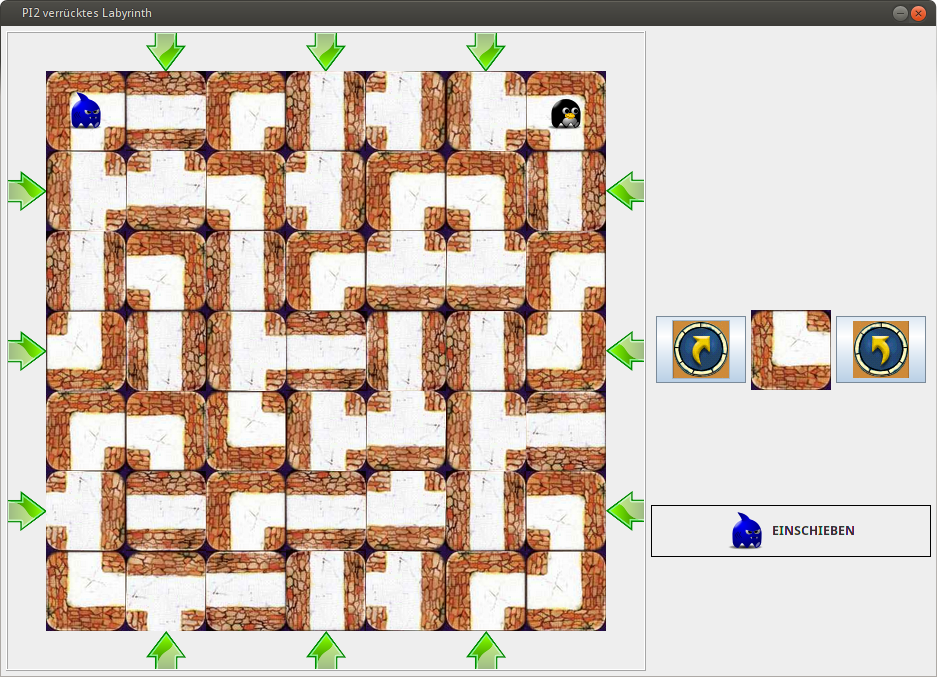
\includegraphics[width=0.8\textwidth]{hauptfenster.png}
  \caption{PI2 verrücktes Labyrinth}
  \label{gui}
\end{figure}

Die SpielerInnen sind nun abwechselnd am Zug, wobei immer diejenige mit der blauen Spielfigur beginnt. 
Zunächst muss das SchiebePlättchen in das Spiel eingeschoben werden. Das geht an all den Stellen, an denen sich im 
Spielfeld ein grüner Pfeil befindet. Wird das Plättchen \zB am Pfeil oben rechts eingeschoben, dann schieben sich 
alle Plättchen in dieser Zeile um eine Position nach links, wobei das Plättchen ganz links aus dem Spielfeld 
herausfällt. Dieses Plättchen wird das neue SchiebePlättchen, das im Zug der nächsten SpielerIn eingeschoben werden 
muss. Das SchiebePlättchen darf vor dem Einschub beliebig gedreht werden (um 90, 180 oder 270 Grad). Eine Spielfigur 
wird \gGF mit ihrem Plättchen verschoben, außer sie wird aus dem Spielfeld geschoben. In diesem Fall wird sie auf das 
gerade eingeschobene Plättchen versetzt.

Nun darf dieselbe SpielerIn ihre Spielfigur auf ein anderes Plättchen setzen (muss das aber nicht). 
Das Zielplättchen darf beliebig weit weg sein, muss allerdings durch einen Weg auf dem Spielfeld vom Ausgangsplättchen 
erreichbar sein (\zB darf die blaue Spielfigur in Abbildung \ref{gui} drei Plättchen weiter nach unten ziehen, die 
schwarze Spielfigur aber nicht zwei Plättchen weiter nach links). Die Spielfeldgrenzen dürfen dabei nicht überschritten 
werden. 

Nach dem Versetzen oder Stehenlassen der Spielfigur ist die andere SpielerIn an der Reihe und muss nun zunächst wieder 
das SchiebePlättchen einschieben.

Sobald eine der beiden Spielfiguren auf ihr entsprechendes Plättchen unten rechts bzw.\ links gesetzt wird, ist das 
Spiel beendet und die SpielerIn dieser Spielfigur hat gewonnen.

\section*{Vorbemerkung}
Ihr findet bei Stud.IP ein gepacktes Eclipse-Projekt \textit{PI2Laby}. In diesem Projekt befinden sich 
mehrere Interfaces und diverse Klassen, die die wesentliche Logik des Spiels und die in Abbildung \ref{gui} 
dargestellte GUI (Graphical User Interface = grafische Benutzeroberfläche) realisieren. 

\section{PushPopy \points{30}}
Im Paket \textit{pi2.uebung01.spec} findet ihr \uA die Interfaces \C{PushPopyInterface}, \C{LiFoInterface} und \C{FiFoInterface}. Diese 
Interfaces beschreiben Schnittstellen für konkrete Sammlungen, die Elemente eines beliebigen Typs aufnehmen können. 
Programmiert eine Klasse, die das Interface \C{LiFoInterface} implementiert und eine weitere Klasse, die das 
Interface \C{FiFoInterface} implementiert. Da es sich bei den Sammlungen um beschränkte Sammlungen handelt, müsst ihr als 
unterliegende Datenstruktur Arrays verwenden, \dH ihr speichert die Elemente der Sammlungen jeweils in einem 
entsprechenden Array ab.

Erzeugt zu beiden Klassen JUnit-Tests und testet damit eure Implementierung. Das Testprotokoll besteht dann nur aus dem 
Ergebnis dieser Tests.

\section{Labyrinth \pointstotal{70}}
\subsection{Plättchen \points{20}}
Die abstrakte Klasse \C{Tile} realisiert eine Oberklasse für die Plättchen, die sich auf dem Spielfeld befinden 
können. Sie fasst die gemeinsamen Attribute und Methoden zusammen und gibt für konkrete Unterklassen die Methode 
\m{boolean hasExit(final Direction pDirection)} vor. Die Aufzählung \C{Direction} definiert die Aufzählungselemente 
\C{NORTH}, \C{EAST}, \C{SOUTH} und \C{WEST}.

Implementiert nun in den drei konkreten Unterklassen \C{Curve}, \C{Straight} und 
\C{Junction} jeweils die Rümpfe der Methode \m{hasExit()}. Diese 
Methode gibt \m{true} zurück, falls das jeweilige Plättchen einen Ausgang in der gegebenen Richtung hat.
Das Ergebnis ist also abhängig von der Orientierung (\dH Rotation) des Plättchens. In 
Abbildung \ref{plaettchenarten} seht ihr die drei Plättchenarten mit der Orientierung \C{Direction.NORTH}.

\begin{figure}[ht]
        \centering
        \begin{subfigure}[b]{0.2\textwidth}
                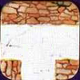
\includegraphics{tplaettchen0.png}
                \caption{Junction}
                \label{fig:tplaettchen0}
        \end{subfigure}
        ~ 
        \begin{subfigure}[b]{0.2\textwidth}
                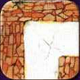
\includegraphics{kurve0.png}
                \caption{Curve}
                \label{fig:kurve}
        \end{subfigure}
        ~ 
        \begin{subfigure}[b]{0.2\textwidth}
                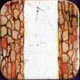
\includegraphics{gerade0.png}
                \caption{Straight}
                \label{fig:gerade}
        \end{subfigure}
        \caption{Die drei Arten von Plättchen}\label{plaettchenarten}
\end{figure}

Für das T-Plättchen in Abbildung \ref{fig:tplaettchen0} liefert die Methode \m{hasExit()} 
nur für den Parameterwert \C{Direction.NORTH} \m{false} zurück, ansonsten \m{true}. Die Orientierung
\C{Direction.EAST} entspricht einer Drehung der Plättchen in Abbildung \ref{plaettchenarten} um 90 Grad im 
Uhrzeigersinn, \C{Direction.SOUTH} um 180 Grad im Uhrzeigersinn und \C{Direction.WEST} um 270 Grad im 
Uhrzeigersinn. Wenn also das Plättchen \m{Curve} aus Abbildung \ref{fig:kurve} die Orientierung \C{Direction.SOUTH} 
hat, dann liefert die Methode \m{hasExit()} für die Parameterwerte  \C{Direction.NORTH} 
und \C{Direction.WEST} \m{true} zurück, ansonsten \m{false}.

Erzeugt JUnit-Tests, die für jede der drei Klassen jeweils die Methode \m{hasExit()} testen. Das Testprotokoll 
besteht dann nur aus dem Ergebnis dieser Tests.

\subsection{Spielfeld \points{50}}
Die Klasse \C{Board} realisiert das eigentliche Spielfeld. Auf dem Spielfeld befinden sich immer 7 Plättchen pro Zeile in 7 Zeilen,
also 7 mal 7 Plättchen (siehe Konstanten in \C{PI2Laby}). Leider fehlt in der Klasse die entscheidende Funktionalität.
Die Methode \m{boolean existsPath(final PieceInterface pPiece, final int pRow, final int pColumn)}, die feststellen soll,
ob die gegebene Spielfigur das Plättchen an den gegebenen Koordinaten erreichen kann, löst in ihrem Rumpf nur eine 
\C{UnsupportedOperationException} aus. Ersetzt den Rumpf durch eine funktionierende Wegfindung.

Dabei wendet ihr folgendes Verfahren an:

Zunächst erzeugt ihr eine Sammlung vom Typ \C{PushPopyInterface} für die noch zu bearbeitenden Plättchen (hier genannt \C{Rand}). 
Fügt jetzt das Plättchen, auf dem sich die gegebene Spielfigur befindet, in die Sammlung \C{Rand} ein. Nun beginnt eine 
Schleife, die so oft wiederholt wird, wie sich noch Elemente in der Sammlung \C{Rand} befinden. Innerhalb der Schleife entnehmt ihr 
mittels \m{pop()} ein Plättchen \C{P} aus dem Rand.  Wenn dieses Plättchen bereits das Ziel ist, seid ihr fertig und könnt \m{true} zurückgeben.
Anderenfalls bestimmt ihr für \C{P} alle Nachbarplättchen, zu denen es einen Weg gibt (\dH ihr müsst für alle Ausgänge von \C{P} das jeweilige
Nachbarplättchen untersuchen und feststellen, ob es einen Ausgang in Richtung \C{P} hat). Diese Nachbarplättchen sind also alle vom aktuellen
Plättchen aus erreichbar (und umgekehrt). Fügt diese Nachbarplättchen daher in die Sammlung \C{Rand} ein. Falls das Zielplättchen nicht 
erreichbar ist, wird es auch niemals als Nachbarplättchen bearbeitet, also nie in den Rand gelangen.  Wenn der Rand dann schließlich leer ist, 
ist eure Schleife beendet und ihr könnt \m{false}  zurückgeben.

Wenn ihr den Algorithmus exakt wie oben umsetzt, kann es passieren, dass die Wegfindung konzeptionell sehr sehr lange dauert \bzW dass euch eure 
\C{PushPopyInterface}-Sammlung auseinanderplatzt. Das liegt daran, dass bereits bearbeitete Plättchen später als Nachbarplättchen erneut in den \C{Rand}
eingefügt werden. Erzeugt daher eine beliebige konkrete Sammlung vom Typ \C{Collection}, die die im Laufe des Algorithmus bereits bearbeiteten 
Plättchen enthält. Ein Plättchen sollte nur dann in den \C{Rand} gelangen \bzW nur bearbeitet werden, wenn es nicht in der Sammlung der bereits
bearbeiteten Plättchen enthalten ist.

Verwendet für den Rand bei der Wegfindung einmal eine Sammlung vom Typ \C{LiFoInterface} und einmal vom Typ \C{FiFoInterface} und 
vergleicht deren Nutzung (in dem ihr \zB die Zahl der Schleifendurchläufe zählt). Gibt es Unterschiede? Erläutert, 
warum es keinen Unterschied macht, welche Datenstruktur eingesetzt wird oder worin die Unterschiede bestehen und wie 
sie zustande kommen.

JUnit-Tests sind hier nicht nötig. Die Tests erfolgen durch Spielen des Spiels: Testet eure Implementierung, in dem ihr ein
oder mehrere Spiele mit der GUI spielt. Protokolliert dabei knapp(!), was funktioniert und was evtl. nicht.

\section*{Hinweise}
Wenn eine SpielerIn die eigene Spielfigur nicht setzen möchte, klickt sie einfach auf das Plättchen, auf dem sich die 
Spielfigur gerade befindet. Dieser Fall sollte also auch getestet werden!

\end{document}
